\documentclass[journal]{IEEEtran}
\usepackage{amsmath,amssymb,amsthm}
\usepackage{booktabs}
\usepackage{graphicx}
\usepackage{cite}
\usepackage{placeins}
\usepackage{url}
\newtheorem{theorem}{Theorem}
\newtheorem{conjecture}{Conjecture}
\begin{document}
\title{How Many Firing Rates Should a Neuron Use? Poisson and Non-Poisson Spike Counts in Long and Short Windows}
\author{I~Made~Tristan~Hope~Firdaus\\
{\normalsize Independent Researcher, Bali, Indonesia}\\
{\normalsize E-mail: madetristanfirdaus@gmail.com\quad ORCID: 0009-0002-3048-3624}}
\maketitle

\begin{abstract}
A stimulus sets a neuron's firing rate anywhere between silence and a peak, and a downstream cell sees only the spike count in a window.
The neuron is then a channel from rates to counts, and the rate is its input. The rate code that carries the most information uses finitely many distinct
rates; how many was known only between order $\sqrt A$ and order $A$, with $A$ the peak count per window. We conjecture, and test
for five to twenty-four rates, that in long windows the number of rates of a Poisson neuron equals the number of levels of the
unit-noise Gaussian channel read at the Fisher half-length $\sqrt A$, shortened by a constant set at silence. The constant follows from
a chain of levels next to silence, with no parameter fitted to the count changes. Certificates in ball arithmetic fix the count at
thirty-five peak counts, up to 66 rates at $A = 2000$, well above a $\sqrt A$ fit to earlier numerics; four count changes were predicted
before they were computed. With a baseline rate the law agrees with twenty-five published count changes with no free parameter, and
neurons more regular or more variable than Poisson add one finite-size term. Without an energy budget the long-window code is on-off up
to $A = 3.3679$ and graded beyond, and at $A = 10$ an on-off code loses at least 24\% of the capacity. Under an energy budget at $A = 3$
the code is graded at some budgets and gains at most 0.8\%. In short windows the normal approximation, maximized by search, chose an
on-off code in all 185 cases computed, many of them outside its accuracy range. At $A = 3$, refractoriness modelled as spike history
leaves the capacity at its Poisson value; modelled as count regularity it raises it. A pre-registered test on six datasets did not find
discrete levels in recorded neurons.
\end{abstract}

\begin{IEEEkeywords}
Capacity-achieving distribution, Poisson channel, neural coding, firing rate, finite blocklength, Fisher information.
\end{IEEEkeywords}

\section{Introduction}
Consider a neuron whose firing rate a stimulus can set anywhere between silence and a peak rate $L$. In a counting window of length
$T$ the neuron emits a random number of spikes with mean $xT$, where $x$ is its current rate, and a downstream reader sees only that
count. The rate is therefore the neuron's input and the count is its output, so the neuron is a noisy channel from rates to counts.
We write $A = LT$ for the peak count, the largest expected number of spikes in one window.

When spikes are counted over many windows, the distribution of rates that carries the most information about the stimulus uses
finitely many distinct rates, one of which is silence~\cite{Shamai1990,IkedaManton2009}. An optimal rate code thus drives the neuron
at a few discrete levels, and theory has predicted discrete tuning curves, from the information they carry~\cite{Nikitin2009} and
from the error of reconstructing the stimulus~\cite{Bethge2003}.
The levels matter for energy as well, because every spike costs ATP~\cite{AttwellLaughlin2001}, and once that cost is counted the code
with the largest capacity is in general not the best one~\cite{LevyBaxter1996}. How many levels the optimal code uses has been known only within wide bounds, between
order $\sqrt A$ and order $A$ for a Poisson neuron~\cite{DBS2021,BDS2024}.

Three features of a real neuron could change that number. Its spike count may be more regular than Poisson, because of
refractoriness, or more variable. It may fire at a baseline rate even when the stimulus asks for silence. The reader may also count
spikes over a window that holds only a few of them, where the asymptotic notion of capacity no longer applies. This paper treats all
three, in the terms of Table~\ref{tab:symbols}; a \emph{count change} is the peak count at which the optimal code gains a rate.
\begin{itemize}
\item In long windows, we conjecture that the number of rates of the optimal code equals the number of levels of the Gaussian
channel with unit noise, read at the half-length $\sqrt A$ shortened by a constant set at silence (Section~\ref{sec:long}). The
constant is computed from a chain of levels next to silence, with no parameter fitted to the count changes, and the conjecture is
tested for five to twenty-four rates. Certificates in ball arithmetic fix the exact count at thirty-five peak counts, up to $66$ rates
at $A = 2000$, and four count changes were predicted before they were computed. The certified counts at large $A$ lie well above a
$\sqrt A$ fit to earlier numerics, which had suggested $\sqrt A$ growth.
\item Neurons more regular or more variable than Poisson carry the same constant at silence, and their counts follow the same law
with one finite-size term (Section~\ref{sec:fano}).
\item A baseline rate moves the constant from its Poisson value to the Gaussian one; with no free parameter, the law reproduces
twenty-five published count changes (Section~\ref{sec:baseline}).
\item Without an energy budget the long-window code is on-off up to the first count change, $A = 3.3679$, and graded beyond it.
The graded code soon carries much more: at $A = 10$ an on-off code loses at least $24\%$ of the capacity. Under an energy budget
at $A = 3$ the code is graded at some budgets and gains at most $0.8\%$ there. For short windows we maximized the normal
approximation to the finite-blocklength rate. For the Poisson neuron and for neurons with a refractory spike history its maximizer was
binary in all $185$ cases computed, at peak counts up to $6$; many of them lie outside the accuracy range of the approximation
(Section~\ref{sec:short}).
\item Refractoriness modelled as spike history cannot change the probability of a silent window, so at $A = 3$, where the optimal
codes are on-off, such a neuron has exactly the Poisson capacity. On the energy--capacity front it lies above the Poisson neuron and
below a count model of similar regularity (Section~\ref{sec:short}).
\item A pre-registered test on six public datasets did not find the predicted levels in recorded neurons (Section~\ref{sec:data}).
\end{itemize}

Most of these statements are measurements. The certified counts are theorems about single peak counts, and one
interval statement follows from them under a published monotonicity conjecture (Section~\ref{sec:long}); the count law itself is a
conjecture supported by the evidence below. Predictions marked as registered were written in a dated, append-only log before the
quantity was computed; the log's time stamps are not certified by a third party. The scripts, the
certificates and the result files are at \url{https://github.com/Tristan-tech-ai/how-many-firing-rates}, and the log is public with
the companion paper's material~\cite{Paper1}.

\emph{What the answer is for, and what it does not show.} For neuroscience the law turns the theory of optimal rate codes into
numbers that can be checked against a neuron. For a neuron with a peak rate of $100$ spikes/s read in windows of $30$~ms ($A = 3$),
the information-maximizing code is on-off. In windows of $100$~ms ($A = 10$) it uses four rates. The change from three to four
rates lies near $A = 9.8$ in the computed optima of Barletta and Dytso~\cite{BarlettaDytso2022}, and a fifth rate first appears at
$A = 18.1$ (Table~\ref{tab:trans}). There the graded code matters: an on-off code carries at most $\log 2$ nats per window, at least
$24\%$ less than the capacity at $A = 10$. At $A = 3$ under an energy budget, where a graded code can also win, it gains less than
$1\%$. In short windows the objective we maximized chose an on-off code in every case, but most of those cases lie where that
objective is inaccurate (Section~\ref{sec:short}). The same channel describes photon counting with a peak-limited light source and
dark counts~\cite{Shamai1990}, where the baseline is the dark-count rate. There the conjectured law predicts the number of intensity levels of
the best pulse-amplitude constellation without solving for it, and it agrees with published dark-current
results~\cite{BarlettaDytso2022}. The test on recorded neurons is negative. Either these neurons do not maximize this
information at the windows tested, or the data had too few trials to show the levels; we cannot tell which. The law concerns one neuron
whose windows are independent uses of the channel. It says nothing about populations, about codes that use spike timing, or about what
a downstream cell actually reads.

\section{The neuron as a channel}\label{sec:model}
The input $x \in [0, A]$ is the expected count produced by the stimulus in one window, the output $Y$ is the count, and $Y \sim
\mathrm{Poisson}(x + \lambda)$, where $\lambda \ge 0$ is the baseline count per window (the dark current of the optics literature).
For an input law $P$ with output mixture $Q$, let $D(x) = D\big(\mathrm{Poisson}(x + \lambda)\,\|\,Q\big)$, the relative entropy that the main text writes $i(x)$; there the letter $D$ is the number of distinct mean counts. Then $P$ achieves the
capacity $C$ if and only if
\begin{equation}
D(x) \le C \ \text{ on } [0, A], \quad \text{with equality on } \operatorname{supp} P,\label{eq:kkt}
\end{equation}
and the optimal $P$ is unique and has finitely many atoms~\cite{Shamai1990,Cao2014}. We write $K(A, \lambda)$ for their number and
$K(A) = K(A, 0)$, as in the main text. The Fisher information of the Poisson count is $1/(x + \lambda)$, so in the Fisher coordinate $t = 2\sqrt{x +
\lambda}$ the noise has unit size everywhere: two rates one unit apart in $t$ are equally hard to tell apart wherever they lie. The
input range has half-length
\begin{equation}
h(A, \lambda) = \sqrt{A + \lambda} - \sqrt{\lambda}.\label{eq:h}
\end{equation}
The reference is the Gaussian channel $Y = X + Z$ with standard normal noise $Z \sim \mathcal N(0, 1)$ and $X \in [-A_g, A_g]$, whose input is discrete at the
optimum~\cite{Smith1971}, whose Fisher coordinate is its input itself and whose half-length is $A_g$. Read in the Fisher coordinate, the
Poisson channel approaches this Gaussian channel at large counts~\cite{Tsiatmas2013}, and Jeffreys' prior, uniform in that coordinate, is
asymptotically capacity-achieving~\cite{ClarkeBarron1994}. We write $N_G(h)$ for its number of levels at half-length $h$, a staircase in $h$, and $A_g(K)$ for the
half-length at which its $K$-th level appears.

Two families describe neurons that are not Poisson. A count more regular than Poisson has Fano factor below one; the binomial count
is the simplest case, with Fano factor $1 - p$ for a success probability $p$ in each trial. A count more variable than Poisson has Fano factor above one, the negative binomial
being the standard case, with Fano factor $1 + \text{mean}/\rho$ for size parameter $\rho$. The Conway--Maxwell--Poisson (COM-Poisson)
family~\cite{Shmueli2005} covers both directions with one shape parameter $\nu$, sub-Poisson for $\nu > 1$ and super-Poisson for
$\nu < 1$, and contains the Poisson count at $\nu = 1$; it is a standard model of spike counts~\cite{Stevenson2016}. Refractoriness can
also be modelled as spike history, by a generalized linear model (GLM) whose conditional intensity is multiplied by
$\exp(\sum_j \eta_j y_{t-j})$, where $y_{t-j}$ marks a spike $j$ bins earlier and $\eta_j$ is the kernel $\eta(s) = -a\,e^{-s/\tau}$ at the lag $s$ of $j$ bins. We use
$\tau = 4$~ms, amplitudes $a = 0$, $2$, $4$ and $8$, and bins of $2$~ms, and the history is reset at the start of each window. A bin
holds at most one spike, so even the kernel $a = 0$ gives a count with Fano factor $0.89$ at a rate of $60$~Hz in $50$~ms windows; the
GLM without history is therefore not the Poisson neuron.

In a short decision the reader does not see many windows. Suppose a message must be decoded from $n$ windows (the blocklength) with
error probability $\epsilon$. In the normal approximation, which drops terms of order $\log n$, the largest number of messages
$M^\ast$ satisfies
\begin{equation}
\log M^\ast(n, \epsilon) \approx nC - \sqrt{nV}\,Q^{-1}(\epsilon),\label{eq:ppv}
\end{equation}
where $V$ is the channel dispersion, the variance of the information density, and $Q^{-1}$ the inverse of the Gaussian tail
function~\cite{PPV2010}. With an energy cost the
same form holds with the cost-constrained $C$ and $V$~\cite{KostinaVerdu2015}. We charge energy linearly in the mean rate, as the
Attwell--Laughlin budget does~\cite{AttwellLaughlin2001}. Table~\ref{tab:symbols} collects the symbols.

\begin{table}[t]\centering\caption{Symbols}\label{tab:symbols}
\footnotesize
\begin{tabular}{@{}p{0.36\columnwidth}p{0.58\columnwidth}@{}}\toprule
symbol & meaning\\\midrule
$x$, $A$ & expected count in a window; peak count, the peak rate times the window\\
$\lambda$ & baseline count per window\\
$K(A, \lambda)$, $N_G(h)$ & number of rates (Poisson); of levels (Gaussian)\\
$h = \sqrt{A + \lambda} - \sqrt\lambda$ & Fisher half-length of the rate range\\
$A_K$, $A_g(K)$ & peak count (Poisson) and half-length (Gaussian) at which level $K$ appears\\
$c(K)$ & wall constant, $\sqrt{A_K} - A_g(K)$\\
$n$, $\epsilon$, $V$ & number of windows, error probability, dispersion\\
\bottomrule\end{tabular}
\end{table}

\section{Long windows: how many rates}\label{sec:long}
\subsection{The count law}
In the Fisher coordinate the levels of the optimal Poisson code are spaced like the levels of the unit-noise Gaussian channel, except
near silence. A silent neuron never spikes, so the output at $x = 0$ is degenerate, and it sits at a finite Fisher distance from the
rest of the range. In the computed optima the levels next to silence form a boundary layer, and the law below treats its effect as an
extra length that changes slowly with $K$. For the Gaussian channel, Wang, Barletta and Dytso~\cite{WBD2025} summarize an argument of
Zhang~\cite{Zhang1994} that the optimal input approaches Jeffreys' prior in the bulk, with a discrete pattern next to the boundary.
Abbott and Machta found
the first levels next to an endpoint at fixed Fisher distances~\cite{AbbottMachta2019}. We conjecture that the Poisson count is the Gaussian count read at a shortened
half-length,
\begin{equation}
K(A, \lambda) = N_G\big(h(A, \lambda) - c(K, \lambda)\big),\label{eq:law}
\end{equation}
where $c(K)$ is the wall constant. Since $K$ is the count being predicted, \eqref{eq:law} is implicit, and we evaluate it at the count
changes $A_K$, where $K$ is known. We call silence a \emph{wall} because the constraint $x \ge 0$ is active there: the level at
silence carries no derivative condition in~\eqref{eq:kkt}. The constant is defined from the measured count changes as $c(K) =
\sqrt{A_K} - A_g(K)$. It can also be predicted without them, from a half-line chain. The chain has one level fixed at silence with a free
weight, thirty free levels, and ten frozen levels of unit weight at spacing $g$ in the Fisher coordinate. That makes $41$ levels in
all, more than the full problem has for $K \le 24$. The chain's equations ask that $D$
take the same value at every free level and at the first frozen one, and that $D' = 0$ at the free levels: $61$ equations for the
$30$ positions and $31$ weights. We solve them once with the Poisson kernel and once with the Gaussian kernel, and define the
\emph{excess} $E(g)$ as the Fisher position of the thirtieth free level in the Poisson chain minus its position in the Gaussian chain.
We call the resulting prediction the \emph{closure}:
\begin{align}
c(K, \lambda) &= \tfrac12 E\big(g_{\rm eff}(K), \lambda\big),\label{eq:closure}\\
g_{\rm eff}(K) &= A_g(K + 1) - A_g(K - 1),\nonumber
\end{align}
where the factor $\frac12$ converts the Fisher coordinate $t = 2\sqrt x$ to the scale of the half-length $\sqrt A$, and $g_{\rm eff}$
is the local spacing of the Gaussian levels at the count change. The chain law $E(g) = 0.9840 - 0.2347\,g$ is a fit to the chain's own
excess on $1.43 \le g \le 2.35$ (root-mean-square deviation $0.0012$); it never sees a count change. The estimator $g_{\rm eff}$ was
chosen among three by comparing them with the measured wall constants; the other two, the one-sided spacing $2(A_g(K + 1) - A_g(K))$
and the mean spacing $2A_g(K)/(K - 1)$, deviate by $0.0043$ and $0.0313$ against $0.0015$ over $K = 5$ to $24$.

A worked case shows how the law is used. For $K = 15$, Table~\ref{tab:trans} gives $A_g(14) = 12.0413$ and $A_g(16) = 13.5819$, so
$g_{\rm eff} = 1.5406$, $E = 0.6224$ and $c = 0.3112$. Adding $c$ to $A_g(15) = 12.8187$ gives $\sqrt{A_{15}} = 13.1299$, against the
measured $13.1302$: the fifteenth rate of the optimal code appears at a peak count of $172.40$. Nothing in that line was fitted to a
Poisson count change.

\subsection{The evidence}
Table~\ref{tab:trans} lists the count changes for $K = 5$ to $24$. The wall constant rises from $0.237$ to $0.335$ with steps that
shrink, and the closure~\eqref{eq:closure} matches it with a root-mean-square deviation of $0.0014$ over $K = 5$ to $20$ and $0.0015$
over $K = 5$ to $24$. The residual follows a smooth trend. It rises steadily from $-0.0026$ at $K = 6$ to $+0.0019$ at
$K = 24$ and changes sign near $K = 14$.

Four count changes were registered before they were computed, each with a tolerance of $\pm 0.15$ in $A$. The twenty-first was
registered at $A = 307.99$ from an earlier local fit of the closure; the full-range law above had been recorded before the computation,
and it gives $308.03$, a number first written down after it. The twenty-second was registered at $333.14$ by the full-range law. The
computation returned $308.09$ and $333.20$. Both residuals, about $+0.0016$ in $c$, matched the size of a finite-length
correction, $+0.002$, that had been estimated beforehand from chains of twenty, thirty and forty free levels, and only then did we
adopt it. With the correction the law placed the next two at $358.97$ and $385.39$, and without it at $358.90$ and $385.31$; both sets
were registered, and the computation returned $358.97$ and $385.38$ (Fig.~\ref{fig:wall}). The law has not been evaluated at the
certified $46$ and $66$ rates of Section~\ref{sec:cert}.

\begin{table}[t]\centering
\caption{Count changes of the Poisson neuron and the wall constant. $A_g$: Gaussian half-length; $A_K$: Poisson peak count;
$c = \sqrt{A_K} - A_g$; closure $E(g_{\rm eff})/2$. Rows 21--24 were predicted before they were computed; the closure column omits
the $+0.002$ correction used for the predictions of rows 23--24. Every $A_g$ is relocated at 128 bits and every $A_K$ comes from the
newborn-weight unfolding at 40 digits.}\label{tab:trans}
\footnotesize\setlength{\tabcolsep}{4pt}
\begin{tabular}{@{}rrrrrr@{}}\toprule
$K$ & $A_g(K)$ & $A_K$ & $c(K)$ & closure & difference\\\midrule
5 & 4.02128 & 18.1366 & 0.2374 & 0.2396 & $-0.0022$\\
6 & 5.05808 & 28.2022 & 0.2525 & 0.2551 & $-0.0026$\\
7 & 6.03983 & 39.7401 & 0.2641 & 0.2666 & $-0.0024$\\
8 & 6.97896 & 52.5995 & 0.2736 & 0.2756 & $-0.0021$\\
9 & 7.88348 & 66.6665 & 0.2815 & 0.2831 & $-0.0016$\\
10 & 8.75901 & 81.8521 & 0.2882 & 0.2894 & $-0.0012$\\
11 & 9.60969 & 98.0839 & 0.2940 & 0.2949 & $-0.0008$\\
12 & 10.43871 & 115.3023 & 0.2992 & 0.2997 & $-0.0005$\\
13 & 11.24859 & 133.4562 & 0.3037 & 0.3039 & $-0.0002$\\
14 & 12.04135 & 152.5025 & 0.3078 & 0.3078 & $+0.0001$\\
15 & 12.81867 & 172.4026 & 0.3115 & 0.3112 & $+0.0003$\\
16 & 13.58195 & 193.1236 & 0.3149 & 0.3144 & $+0.0006$\\
17 & 14.33238 & 214.6348 & 0.3180 & 0.3173 & $+0.0008$\\
18 & 15.07098 & 236.9105 & 0.3209 & 0.3199 & $+0.0010$\\
19 & 15.79863 & 259.9251 & 0.3236 & 0.3224 & $+0.0011$\\
20 & 16.51609 & 283.6578 & 0.3261 & 0.3247 & $+0.0013$\\
21 & 17.22406 & 308.0874 & 0.3284 & 0.3269 & $+0.0015$\\
22 & 17.92312 & 333.1959 & 0.3305 & 0.3289 & $+0.0016$\\
23 & 18.61381 & 358.9655 & 0.3326 & 0.3308 & $+0.0018$\\
24 & 19.29662 & 385.3810 & 0.3345 & 0.3326 & $+0.0019$\\
\bottomrule\end{tabular}
\end{table}

\begin{figure}[t]\centering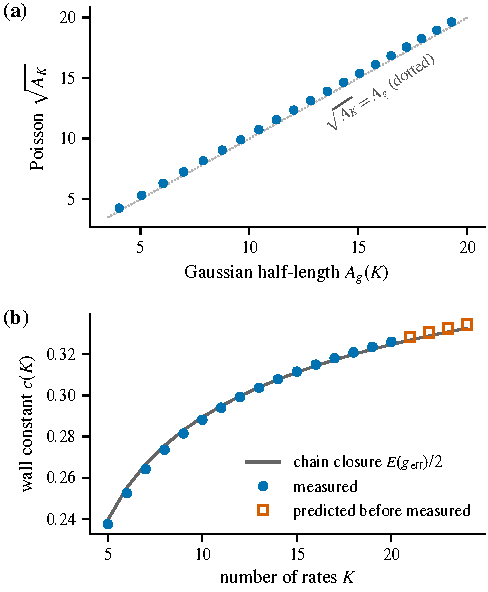
\includegraphics[width=\columnwidth]{figs/fig_wall.pdf}
\caption{The Poisson count is the Gaussian count at a shortened Fisher half-length. (a) Poisson count changes $\sqrt{A_K}$ against the
Gaussian ones $A_g(K)$, $K = 5$ to $24$: a line of slope one, offset by the wall constant. (b) The wall constant $c(K)$, measured (dots)
and predicted by the chain closure (line); open squares, $K = 21$ to $24$, were predicted before they were computed.}\label{fig:wall}
\end{figure}

\subsection{Certified counts}\label{sec:cert}
The count itself was certified at thirty-five peak counts. For each, the optimality condition~\eqref{eq:kkt} was proved over the whole
range $[0, A]$ in ball arithmetic for one computed input~\cite{Johansson2017}, and since the optimal input is unique this fixes $N(A)$
exactly. Thirty-two certificates cover $A = 27.9$ to $378$ with five to twenty-three rates, none at nine (Appendix~\ref{app:cert}); among
them the smallest margin by which $D$ stays below $C$ off the support is $3.3\times 10^{-13}$, at $K = 22$. Three later certificates
give $21$ rates at $A = 311.37$, $46$ at $A = 1144.25$ and $66$ at $A = 2000$, with margins $1.9\times 10^{-20}$, $1.8\times 10^{-25}$
and $1.8\times 10^{-29}$. These are theorems about single peak counts. One statement about intervals follows
if the count never falls as $A$ grows. For the peak-limited Gaussian channel Sharma and Shamai describe this monotonic growth as
commonly assumed but open, and they assume that the count grows by at most one point at a time~\cite{SharmaShamai2010}.

\begin{theorem}[conditional on monotonicity]\label{thm:intervals}
If $N(A)$ is non-decreasing, then $N(A) = K$ on each of the eleven intervals between the smallest and largest certified peak counts
with the same $K$ in Table~\ref{tab:cert}; together they cover $170.4$ of the $350.1$ in $A$ spanned by these certificates.
\end{theorem}
\begin{proof}
If $N(a) = N(b) = K$ with $a < b$, then $K = N(a) \le N(A) \le N(b) = K$ for every $A \in [a, b]$.
\end{proof}
The later certificate of $21$ rates at $A = 311.37$ lies inside the interval for $K = 21$, as the theorem requires. The published
staircases of Barletta and Dytso~\cite{BarlettaDytso2022} show no fall in $6430$ consecutive pairs at four baselines, $1320$ of them
without a baseline. These are numerical optima on a grid of step $0.1$ in $A$, up to $A = 127.5$ without a baseline, so a narrower dip
would not be seen. Across the $230$ consecutive pairs of high-precision states on the nine plateaux we sampled, neither the smallest
gap between rates nor the smallest weight ever decreases. A fall would need one of them to reach zero, so this argues against a fall,
but it is not a proof.

\subsection{How fast the count grows}
The law~\eqref{eq:law} carries the growth of the Gaussian count to the Poisson neuron. Abbott and Machta derive, from a continuum
ansatz and without proof, that the Gaussian count grows as $L^{4/3}$ at half-length $L$~\cite{Mattingly2018,AbbottMachta2019}.
Through the Fisher length the Poisson count would then grow as $A^{2/3}$. The best proved bounds on the Gaussian count are of order
$L\sqrt{\log L}$ from below and $L^2$ from above~\cite{WBD2025,DYPS2020}. In the companion paper the leading constant is measured, as
$0.4002$, in three problems~\cite{Paper1}, so the Poisson neuron should use about $0.4002\,A^{2/3}$ rates at large $A$. This gives
$18.4$, $43.8$ and $63.5$ at the three later certificates, against the certified $21$, $46$ and $66$; the Gaussian count exceeds its own
leading term by a similar amount, about three levels at its count changes $L = 12.82$ and $19.30$. From numerical optima up to
$A = 128$, Barletta and Dytso
conjectured that the Poisson count grows as $\sqrt A$~\cite{BarlettaDytso2022}, the order of a lower bound that Dytso, Barletta and
Shamai had conjectured to be tight~\cite{DBS2021}. A $\sqrt A$ law fitted to those optima for $A \ge 20$ gives $37$ and $49$ rates at
$A = 1144.25$ and $2000$, against the certified $46$ and $66$, while an $A^{2/3}$ law fitted to the same optima gives $47$ and $68$. No
finite range settles an asymptotic order, but over this range the counts follow $A^{2/3}$ more closely than $\sqrt A$. A proof that the count is at
least $cA^{2/3}$ for every $c < 0.0117$ and all $A$ beyond a threshold, which is not computed and is very large, is the subject of
separate work and is not used here.

At the other end, the count changes first from two rates to three at $A = 3.3679$, a threshold that Barletta and
Dytso~\cite{BarlettaDytso2022} attribute to Shamai~\cite{Shamai1990}: below it the best code is on-off, silence and the peak rate. For mutual information, Bethge et al.\ noted
without showing the computation that a binary code stays optimal up to a peak count of about $3.5$~\cite{Bethge2003}, and conditions
for binary inputs with a baseline or an average-power constraint are in~\cite{Cao2014b}. We recomputed $3.3679$ from the interior
optimality condition of the best binary input. Section~\ref{sec:short} returns to it.

\section{Neurons more regular or more variable than Poisson}\label{sec:fano}
A neuron more regular or more variable than Poisson keeps the wall at silence. The binomial and negative-binomial counts both have a
degenerate output at silence, at a finite Fisher distance, and the first two \emph{gaps} next to silence, the spacings between
neighboring rates in the Fisher coordinate~\cite{Anscombe1948}, are the Poisson ones: $3.126$ and $2.260$ Fisher units for the binomial
with $n_b \ge 1000$ trials, and $3.125$ and $2.260$ for the negative binomial with size $\rho = 1000$. These place the first two levels
above silence at $3.13$ and $5.39$; Abbott and Machta found $3.13$ and $5.41$ for the Poisson count~\cite{AbbottMachta2019}. Unlike the Poisson count, whose
variance equals its mean, these counts have a variance-to-mean ratio that changes with the rate, and that adds one term. Writing
$q(x) = \sqrt{\text{mean}/\text{variance}}$ and $q_0 = q(0)$, the count is read at the effective half-length
\begin{equation}
h_{\rm eff} = h_F - \kappa\,\frac{h_F - q_0\sqrt A}{K},\label{eq:heff}
\end{equation}
where $h_F$ is the Fisher half-length, $A$ the peak count and $\kappa = 0.42 \pm 0.02$ a measured constant. It comes from 54 count changes of the
binomial count on $[0, \varrho n_b]$, a fraction $\varrho$ of its full range with peak count $A = \varrho n_b$ and one wall ($K = 9$,
$11$, $17$ and $18$). Seven more come from the binomial channel on its full range, where both ends are walls ($K = 18$ to $24$). Six
count changes of the negative binomial give $0.39$. The term vanishes for the Poisson count and for any count whose variance-to-mean ratio is
constant, as the generalized Poisson count of Consul confirms ($|\Delta h| < 0.0005$). It also vanishes as $K \to \infty$, so the
Fisher-length law is its large-$K$ limit. Registered before they were computed, \eqref{eq:heff} placed the 25th and 26th count changes
of the full-range binomial channel at $n_b = 174.94$ (with $\kappa = 0.435$, the value measured at the time) and $186.36$ (with
$\kappa = 0.42$). The registered ranges for $\kappa$ from $0.40$ to $0.46$ were $174.76$--$175.07$ and $186.24$--$186.55$, and the
solver returned $174.934$ and $186.386$. At $\kappa = 0.42$ the two predictions are low by $0.07$ and $0.04$. For the binomial channel, the published bounds on the count and the computed optimal inputs are
in~\cite{Zieder2024,Favano2026,Baniasadi2026}.

The COM-Poisson neuron also has a degenerate output at silence, so the same construction predicts its count, with its own Fisher length
and dispersion ratio; we have not computed its wall constant. What we did compute is its count at Fano factors $0.9$, $1.13$, $1.3$
and $1.5$, which bracket the median Fano factors of the datasets of Section~\ref{sec:data} ($0.90$ to $1.12$, and $1.39$ in V1). For
$A \le 12$ it differs from the Poisson count by at most one rate, and variability above Poisson never raises it. In long windows, then, the number of rates is a property of the Fisher length of the rate range
and of the type of the endpoint at silence. A neuron's Fano factor enters only through these and, at finite $K$, through the
dispersion ratio at silence in~\eqref{eq:heff}.

\section{A baseline rate}\label{sec:baseline}
A baseline rate removes the degenerate output: with $\lambda > 0$ a silent stimulus still produces spikes, and the endpoint at silence
becomes regular. The wall constant then falls from its Poisson value toward the Gaussian value, zero; at $K = 11$ it is $0.29$ at
$\lambda = 0$ and $0.02$ at $\lambda = 1$. The chain with the same kernel predicts this crossover with no parameter, to $0.002$ at
$K = 11$ (six baselines) and to $0.001$ at $K = 15$ (three). In the Fisher offset of the endpoint, $d = 2\sqrt\lambda$, the change is
linear at small $d$, $E(g, 0) - E(g, \lambda) = 1.06\,d$, and the remaining excess decays as $0.055/d$ at large $d$; a baseline of
$10^{-3}$ spikes per window already removes a tenth of the wall.

The law~\eqref{eq:law}--\eqref{eq:closure} with this chain predicts the twenty-five count changes in the published optimal inputs of
Barletta and Dytso~\cite{BarlettaDytso2022} for $\lambda = 1$, $10$ and $100$ (nine, eight and eight changes, from three rates up to
eleven). The root-mean-square deviations are $0.005$, $0.004$ and $0.003$ in the Fisher half-length, and the largest is $0.009$. The six
changes to three and four rates lie below $K = 5$, where $g_{\rm eff}$ exceeds the range on which the chain law was fitted; for them the
agreement is with the law's extrapolation. The chain also gives the second rate
of the code: its first gap $g_1$ next to silence places it at an expected count of $(g_1/2 + \sqrt\lambda)^2 - \lambda$ above the
baseline. This is $4.64$, $10.48$ and $29.06$, against the published $4.64$, $10.49$ and $29.06$ at the largest peak count of each run. For every baseline the
lowest rate of the optimal code stays at silence, where the neuron fires at the baseline rate. Where a new rate appears is also set
at silence. An inserted rate appears at $0.62$ of its gap from the silent side, and a split happens at $0.12$ of the gap next to the
parent rate, against $\frac12$ and $0$ for the Gaussian channel. The baseline carries both values to the Gaussian ones
(Appendix~\ref{app:birth}).

\section{Short windows}\label{sec:short}
\subsection{A window that holds few spikes}
Spike counts are commonly computed in windows of about $50$~ms~\cite{Churchland2010}, and such a window often holds only a few spikes.
There the asymptotic capacity overstates what a neuron delivers; Kostal and Shinomoto found a drop of about an order of magnitude under
finite coding~\cite{KostalShinomoto2016}. By~\eqref{eq:ppv}, the relative loss $\phi = \sqrt{nV}\,Q^{-1}(\epsilon)/(nC)$ of a Poisson
neuron depends mainly on the expected number of spikes $N_{\rm sp}$ in the whole decision, $\phi \approx Q^{-1}(\epsilon)/\sqrt{N_{\rm
sp}}$~\cite{Firdaus2026a}. The approximation holds when $C^2/V$ is close to the mean count per window, since $\phi =
Q^{-1}(\epsilon)\sqrt{V/(nC^2)}$. In the windows used here $C^2/V$ is about $12\%$ above the mean count (at $A = 3$, $C = 0.5944$ and
$V = 0.2224$ nats, so $C^2/V = 1.59$ against a mean count of $1.41$). In continuous time with a slack power constraint the two are
equal~\cite{SakaiTanKovacevic2020}; when an energy budget binds they are not, and the approximation fails. At $\epsilon = 0.01$, where
$Q^{-1}(\epsilon) = 2.33$, a decision built on fifty spikes loses a third of the asymptotic rate. With fewer than about sixty spikes
$\phi$ exceeds $0.3$, where the expansion is no longer accurate and overstates the loss, but the loss stays large. Below a total of
about $Q^{-1}(\epsilon)^2 = 5.4$ spikes the right side of~\eqref{eq:ppv} is negative, that is, less than one message can be decoded
reliably, a known consequence of the expansion.

\subsection{The best short-window code is on-off}
The loss also changes which code is best. Bethge, Rotermund and Pawelzik found binary tuning optimal for rate coding at high temporal
resolution~\cite{Bethge2003}; here the objective is the right side of~\eqref{eq:ppv}, and the comparison is with the exact long-window
optimum. We maximized that objective by search over input laws on a grid of rates from $0$ to $60$~Hz, for the Poisson neuron and for
the four GLM kernels of Section~\ref{sec:model} (induced Fano factors $0.89$ to $0.46$). There were $130$ cases over energy budgets and
blocklengths $n = 10$ and $50$ at $A = 3$, in windows of $50$~ms. Another $55$ were at a fixed decision time of $500$~ms, with windows of $10$ to
$100$~ms, that is, peak counts from $0.6$ to $6$ and $n$ from $50$ down to $5$; eleven of them were for the Poisson neuron. In all $185$
cases the maximizer was binary: silence and one firing rate. A graded law was open to the search in every case and was never chosen.
Three limits apply. The maximizer was found by search and is not certified. The cases at $n = 10$ and all $55$ at fixed decision time
hold at most $30$ expected spikes per decision, so $\phi \approx Q^{-1}(\epsilon)/\sqrt{N_{\rm sp}}$ is at least $0.4$ there, outside
the accuracy range of~\eqref{eq:ppv}. And in many cases
the long-window code is on-off as well, so they cannot show a contrast: at fixed decision time only the peak counts $3.5$, $4.5$ and $6$
exceed the first count change of the Poisson neuron. An exact finite-blocklength bound for a few cases would show whether the on-off
choice survives outside the approximation.

The long-window optimum behaves differently. Without an energy budget it is binary up to $A = 3.3679$ and graded beyond, so it changes
at the first count change of Section~\ref{sec:long}, and beyond it the graded code soon carries much more than any on-off code. An
on-off code carries at most $\log 2 = 0.693$ nats per window, while the capacity is at least $0.762$ nats at $A = 6$, $0.916$ at
$A = 10$ and $1.106$ at $A = 18$ (Blahut--Arimoto on $601$ rates). An on-off code therefore loses at least $9\%$, $24\%$ and $37\%$ of the
capacity there, and at $A = 4$ the best on-off code loses $1.1\%$. With an energy budget the code can be graded at smaller peak counts. At $A = 3$ we
compared the Blahut--Arimoto optimum with every binary code on a $0.5$~Hz grid and call a budget graded when the former exceeds the
latter. For the neuron without spike history the long-window optimum is graded at budgets from $4.4$ to $20.2$~Hz
(Fig.~\ref{fig:graded}). Over the four kernels, $42$ of $83$ distinct budgets are graded in this sense. At the others the Blahut--Arimoto
value falls up to $1.5\times 10^{-4}$ nats below the best binary code, so a graded optimum there is neither shown nor excluded.
Where a graded code was found it gains at most $3.8\times 10^{-3}$ nats per window over the best binary code, $0.8\%$ of the
cost-constrained capacity at that budget. Near $A = 3$ the objective is nearly flat between graded and on-off codes, so a small dispersion
term is enough to tip the choice to on-off. A prediction that rests on a nearly flat objective is fragile, and at $A = 3$ we report the
effect as a change in which code is optimal; the information at stake there is small.

\begin{figure}[t]\centering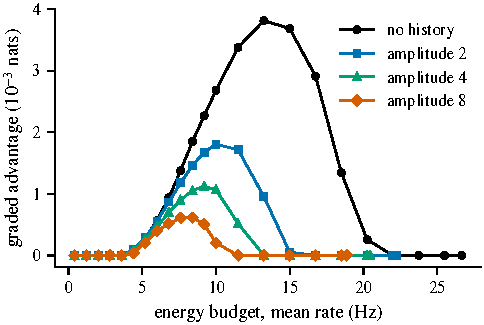
\includegraphics[width=\columnwidth]{figs/fig_graded.pdf}
\caption{Under an energy budget the long-window code can be graded below the first count change, but it gains little. Peak count
$A = 3$ (60~Hz, 50~ms windows): advantage of the Blahut--Arimoto optimum over the best binary code on a $0.5$~Hz grid, for a neuron
without spike history and refractory amplitudes $a = 2$, $4$, $8$ ($\tau = 4$~ms); zero means that no graded code was shown. The
maximizer of the normal approximation was binary in every case.}\label{fig:graded}
\end{figure}

For a physiologist the switch is a statement about two numbers, the peak rate and the counting window. Without an energy budget the
long-window code is graded only when the peak count exceeds $3.3679$, which at a $50$~ms window needs a peak rate of $67$~Hz. Driven layer-4 neurons of
awake trained animals fire at a mean of $12$~Hz, and at $28.5$~Hz one standard deviation above that mean~\cite{BarthPoulet2012}, below
that, while high-rate cells or long counting windows can pass it. Without an energy budget, a neuron that cannot pass it uses the on-off
code in long windows, and the short-window objective chose on-off as well.

\subsection{Refractoriness as spike history and as count regularity}
A refractory kernel acts only after a spike. When the history is reset at the start of each window, the probability of a silent window
is therefore $e^{-x}$ for every kernel, the void probability of a process with an empty history~\cite{DaleyVereJones2003}. Here $x$ is the expected count of the window; at $x = 3$
we computed $0.04978707 = e^{-3}$ for all four kernels. With an on-off code any count above zero identifies the active rate, so the
information depends on the kernel only through that probability. At $A = 3$, where the capacity-achieving code of each of the four GLM
channels is on-off (computed), every GLM neuron therefore has exactly the Poisson capacity, $0.5944$ nats per window. Above the first
count change the Poisson optimum is graded and the identity says nothing. For their continuous-time channel, Kostal and Shinomoto
conclude more generally that a non-Poissonian neuron cannot increase the capacity through causal feedback, provided that the input
satisfies their peak and average constraints and that the spontaneous activity is Poissonian~\cite{KostalShinomoto2016}. The
silent-window identity is the mechanism in our setting. A dead time at the detector is a different model: in the low-power regime it
leaves the leading term of the discrete-time Poisson capacity unchanged unless it limits the output rate~\cite{Wang2020Entropy}. The
capacity per unit cost of a refractory counting model is studied in~\cite{Nasiraee2025}. Spike timing inside the window adds at most $2.7\times 10^{-4}$ nats per window over the count, so the count is
nearly sufficient.

Refractoriness does lower the energy cost, because it suppresses spikes: the realised rate of the top symbol falls from $56.5$ to
$40.0$~Hz as the kernel strengthens. At a matched mean rate between $3$ and $25$~Hz, in long windows, the GLM neuron with induced Fano
factor $0.46$ therefore beats the Poisson neuron, by up to $0.072$ nats per window near $10$~Hz and by $0.006$ at $25$~Hz. A COM-Poisson
count of similar Fano factor ($0.5$) does better again, by $0.026$ to $0.117$ nats per window over the GLM neuron, because it also
lowers the probability of a silent
window, which the GLM leaves at its Poisson value. At Fano factor $0.5$ and a mean count of $2.83$ that probability is $0.0089$, against
$0.059$ for a Poisson count of the same mean. Refractoriness as spike history and as count regularity therefore behave differently, and a count model of a
refractory neuron overstates what refractoriness buys (Fig.~\ref{fig:front}(b)).

\subsection{The energy--capacity front}
The energy--capacity front plots the best information per window against the mean firing rate it costs; Kostal and Shinomoto drew it
for the Poisson neuron on the Attwell--Laughlin axis~\cite{KostalShinomoto2016}, and energy--information trade-offs of neurons go back
further~\cite{LevyBaxter1996,Balasubramanian2001,BergerLevy2010}. For long windows the front is the capacity--cost function, computed by cost-constrained Blahut--Arimoto, so each point is a global optimum. For short windows the front was
found by search over input laws under a direct constraint on the mean rate. A Lagrangian sweep cannot replace the direct constraint here:
the short-window objective is not concave in the input, and at $n = 10$ a sweep over 121 multipliers never reaches rates between
$5.32$ and $22.34$~Hz. Fig.~\ref{fig:front}(a) shows both fronts for COM-Poisson neurons with Fano factors from $0.3$ to $2$; both rise
smoothly with the energy budget. Lower Fano factor is better at every energy but one in each front. In short windows it is better at 43 of 44
comparable energies; the exception is Fano factors $1.5$ and $2$ at $n = 50$ and $3.6$~Hz, which survived a tenfold finer search.
In long windows the same pair is reversed at $0.4$~Hz. The dispersion term thus does not reorder the neurons. The efficient operating point moves, however. The Attwell--Laughlin budget adds a static cost to the cost per
spike. On it, the information per ATP of the Poisson neuron in long windows is largest at $1.2$~Hz on the grid of budgets computed,
whose neighbouring points are $0.4$ and $2$~Hz. That is near the mean rate of about $4$~Hz that the Attwell--Laughlin budget assumes~\cite{AttwellLaughlin2001}.
With $50$ windows the information per ATP is largest near $10$~Hz. Short decisions thus push the efficient rate up, away from the measured rates. For
a single neuron the binding variable is the number of spikes in the decision, which points to pooling or to longer integration.

\begin{figure}[t]\centering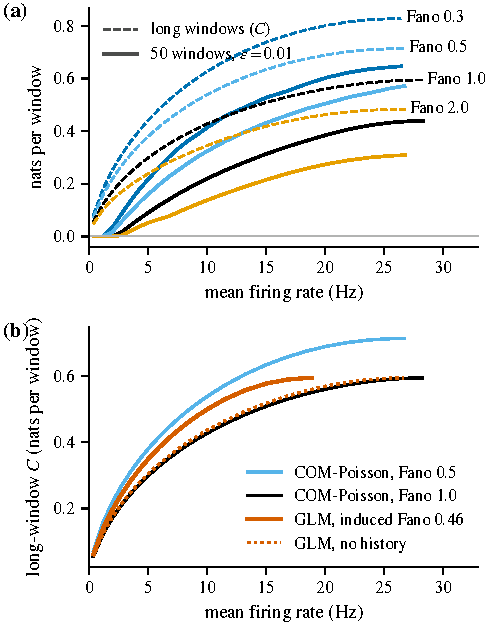
\includegraphics[width=\columnwidth]{figs/fig_front.pdf}
\caption{The energy--capacity front of a neuron. (a) COM-Poisson neurons with Fano factors $0.3$ to $2$: long-window capacity (dashed)
and the short-window front with $50$ windows at $\epsilon = 0.01$ (solid, $\log M^\ast$ per window). Lower Fano factor is better at every
energy but one in each front (43 of 44 in short windows). (b) Long-window fronts of COM-Poisson neurons and of GLM neurons: refractory spike history lies above the Poisson neuron
but below a count model of similar regularity. Windows of $50$~ms, rates $0$ to $60$~Hz.}\label{fig:front}
\end{figure}

\subsection{What Kostal and Shinomoto found, and what changes here}
Kostal and Shinomoto computed the energy--capacity trade-off of a Poisson neuron with the Attwell--Laughlin cost, together with a version
for finite coding at fixed error probability~\cite{KostalShinomoto2016}. They also asked whether, under some coding constraint, a
continuously varied rate might help; the graded long-window codes above are one answer, with a small gain at $A = 3$ and a large one
beyond the first count change. Three differences in the setup
explain the differences in the results. First, their input may switch freely in continuous time, which makes the on-off code optimal; we
hold the rate fixed through a window, and only this restriction allows a graded code at all. Second, they cap the peak rate at $50$~Hz to
keep the linear cost model and the Poisson approximation valid. At a $50$~ms window that cap is $A = 2.5$, below $3.3679$, so without an
energy budget our long-window code is on-off there as well; their model carries an average-power constraint besides the peak, their
Eq.~(2), and with a budget
our code can be graded at $A = 3$ (Fig.~\ref{fig:graded}), so whether it is graded at $A = 2.5$ under their budget is not settled
here. Third, their finite-coding version comes from an error exponent: the window grows until a target error is reached, a
bandwidth-type constraint under which a low rate is paid for with time, and their efficient operating point moves to lower cost. Ours
fixes the number of windows, a blocklength-type constraint that penalizes low rates instead, and the efficient point moves to higher
rates. The two constraints bound the operating point from opposite sides. Our neuron family is also wider, since the COM-Poisson count
covers both directions of variability and contains their Poisson neuron as one member.
\section{Do recorded neurons use discrete levels?}\label{sec:data}
Two lines of theory predict that a single neuron's tuning curve takes a few discrete values~\cite{Bethge2003,Nikitin2009}. Nikitin
et al.\ note that it is not clear whether a test with the right stimulus and counting window has been done, and Bethge et al.\ cite
evidence for binary coding in some neurons, such as the H1 neuron of the fly. We ran a pre-registered test on six public datasets: motor cortex, area 2 and dorsomedial frontal
cortex of monkeys (DANDI 000128, 000127, 000130~\cite{Pei2021}), larval salamander retina (Dryad 10.5061/dryad.4qrfj6qm8), mouse V1
(Allen Visual Coding Neuropixels, DANDI 000021) and mouse A1 (DANDI 000986). For each tuned unit the tuning map was estimated from the
trials, and the number of levels was the number of k-means clusters of that map that best predicts held-out trials. If the code were
discrete, this number would stop growing once enough trials were added. Two comparators were built on each unit: a discrete one, with
$K(A, \lambda)$ levels on the unit's own map and matched noise, and a continuous one, with the map itself and the same noise. Only
units whose two simulations separate are scored, and a shuffle control must give one level.

The registered rule returned \emph{mixed} in five datasets and \emph{smooth} in the salamander retina (Table~\ref{tab:data}). The rule
counts pairs whose level count is one, units without resolvable tuning, as flat, so we also report a second reading restricted to tuned
pairs (level count at least two). There the level count grew with the number of trials in 57 to 85\% of the tuned pairs of five
datasets; in mouse A1, where the count is capped at five levels, 70\% of the tuned pairs reached all five. In M1 and V1 the
\emph{mixed} verdict came from the untuned pairs, since growth among tuned pairs reached 79\% and 85\%; in area 2 and DMFC growth stayed
below 70\% even among tuned pairs. At the full trial count the level count was $1.8$ to $3.3$ times the discrete comparator. It was
within $0.2$ of the continuous comparator in two datasets and differed from it by $1.5$ to $2.0$ levels in the other four, in both
directions. The comparators therefore calibrate the test only to about two levels. Among powered pairs with a peak count below $3.4$, where the
theory predicts two levels, only 2 to 15\% stopped at two. The A1 recordings, with a median peak count of $0.35$ per window among
powered units and a predicted two levels for every one of them, are the case most favourable to the theory. The theory says what the
levels would be if a neuron implemented the optimal code; these recordings do not show them.

\begin{table}[t]\centering\caption{The level-count test on six public datasets}\label{tab:data}
\footnotesize\setlength{\tabcolsep}{2.5pt}
\begin{tabular}{@{}p{0.24\columnwidth}lrlrr@{}}\toprule
dataset & rule & units & levels$^{b}$ & growth & at 2\\\midrule
M1 (MC\_Maze) & mixed & 178 & 8.86 / 2.71 / 8.73 & 79\% & 2\%\\
area 2 & mixed & 65 & 8.10 / 3.02 / 6.63 & 57\% & 9\%\\
DMFC & mixed & 53 & 5.39 / 2.96 / 7.40 & 59\% & 15\%\\
salamander retina & smooth & 381 & 6.55 / 3.10 / 8.43 & 75\% & 10\%\\
mouse V1 & mixed & 100 & 6.46 / 2.67 / 7.92 & 85\% & 8\%\\
mouse A1 (ceiling 5) & mixed & 123 & 4.26 / 2.28 / 4.09 & 70\%$^{a}$ & 8\%\\
\bottomrule
\multicolumn{6}{@{}p{\columnwidth}@{}}{rule: registered verdict; units: powered units; levels: mean level count over powered pairs,
$^{b}$data / discrete comparator / continuous comparator; growth: among tuned powered pairs (level count at least two); at 2: plateau
at two levels among powered pairs with $A + \lambda < 3.4$. $^{a}$Tuned pairs reaching all five levels.}
\end{tabular}
\end{table}

\section{Discussion}
On the evidence for five to twenty-four rates, the number of rates an optimal neuron uses in long windows is a Fisher-length quantity.
The Poisson count is then the Gaussian count at the Fisher half-length $\sqrt A$ shortened by a wall constant, and the constant is half
the extra length that a chain of levels needs next to silence. The neuron's statistics enter only through the type of its endpoint at silence: a degenerate output at finite Fisher
distance gives the Poisson wall, a regular endpoint the Gaussian one. A baseline rate turns the first type into the second, and a
neuron more regular or more variable than Poisson keeps the Poisson wall and adds one finite-size term. For a rate code this means that a
neuron with peak count $A$ and baseline $\lambda$ uses $N_G(\sqrt{A + \lambda} - \sqrt\lambda - c)$ distinct rates. Its lowest rate
is silence, where it fires at the baseline rate, and its second rate sits $(g_1/2 + \sqrt\lambda)^2 - \lambda$ spikes per window
above the baseline, $4.6$ for $\lambda = 1$.

In short windows the normal approximation chose the on-off code, silence and one rate, in every case we computed, though most of
those cases lie outside its accuracy range. The long-window code becomes graded past the first count change, where it soon carries
much more than any on-off code: at $A = 10$ an on-off code loses at least $24\%$ of the capacity. It also becomes graded at smaller peak counts when energy is
scarce, but at $A = 3$ it gains less than one per cent there. Near the first count change the finite-window correction thus changes which code is optimal more than
it changes how much information the code carries. For neurons that are more regular than Poisson, at $A = 3$, the way the regularity is
modelled matters: as spike history it leaves the capacity unchanged, as count regularity it raises it.

This work has the following limits. The wall constant is measured from the chain, and the chain law is an interpolation on $1.43
\le g \le 2.35$, extrapolated by $0.02$ to $0.09$ in $g$ for $K = 21$ to $25$ and above its range for the count changes to three and
four rates. Neither is derived yet. The count law is a conjecture tested for $K = 5$ to $24$ and supported by certificates at single peak
counts; it has not been evaluated at the certified $46$ and $66$ rates. The short-window fronts and maximizers come from a search and
carry no certificate, and every short-window case with at most about $60$ expected spikes per decision, including all at $n = 10$, lies
past the clean validity of~\eqref{eq:ppv}. Windows are treated as independent uses of the channel, so a GLM's history is reset at each window.
In the data, the test asked a narrow question, and a negative answer does not show that neurons ignore energy or information.

Four results would contradict these conclusions. The first is a certified count change at $K = 25$ outside the registered tolerance of
$\pm 0.15$ in $A$ around $A = 412.43$; this prediction was made on 9 September 2026 and has not yet been computed. The others are a
discrete level count in a spike dataset with enough trials, a count whose variance-to-mean ratio varies and that misses~\eqref{eq:heff}
by more than $0.02$ in the half-length, and a graded short-window optimum under an exact finite-blocklength bound.

\emph{What comes next.} The wall constant is measured but not yet derived. A derivation would make the count law a statement about every
channel whose output degenerates at silence. A dataset with many trials per stimulus, counted in short windows, would decide whether
neurons use discrete levels. Behind both sits a broader question that this paper does not settle. The companion paper~\cite{Paper1}
proposes that the optima of capacity, minimax estimation and the NPMLE under Gaussian noise follow one description of the same kind, a
count set by a length and shortened at an edge. Whether the description extends from single neurons to populations, and from counts to
spike timing, is open. If it does, the number of distinguishable responses of a neural population could be read from its noise and
its range in the same way.


\section*{Acknowledgment}
The author thanks Sarah Marzen for helpful comments.

\emph{Use of AI.} Claude (Anthropic) was used as an assisting tool during the preparation of this manuscript, primarily for
computational support and language editing. The research questions, mathematical ideas, methodology, interpretation of results, and
overall direction of the work were developed by the author. All computational results and certificates reported in the manuscript
were recomputed and verified by the author, and the cited works were checked by the author. The author is responsible for the content
and conclusions of this work.

\appendices
\section{Certificates}\label{app:cert}
For a candidate input the optimality equations, $D(x_k) = C$ at all $K$ levels and $D'(x_k) = 0$ at the $K - 2$ interior ones, together
with $\sum_k w_k = 1$, are $2K - 1$ equations in the $K$ weights, the $K - 2$ interior positions and $C$. They were solved by Newton's
method at fifty digits, and the solution was enclosed by a Krawczyk test with an analytic interval Jacobian~\cite{Krawczyk1969}.
Then $D(x) \le C$ was verified on $[0, A]$ in three pieces: a lemma on $(0, 10^{-8}]$, cubic bounds around each level, and chord bounds with
enclosed curvature on every remaining cell. The output alphabet is truncated at $A + 18\sqrt A + 50$ counts and the discarded tail is
enclosed. The box has radius $10^{-28}$ or less, far below the smallest gap and the smallest weight, so the enclosed input has exactly $K$
distinct levels with positive weights. Table~\ref{tab:cert} lists these thirty-two certificates.

The three later certificates use a second pipeline. The alphabet is truncated at $A + 16\sqrt A + 60$ counts for $A =
311.37$ and $1144.25$ and at $A + 20\sqrt A + 60$ for $A = 2000$, and a separately proved lemma bounds the effect of the discarded tail,
so the statement holds for the untruncated channel. The Krawczyk boxes have radii $10^{-22}$, $10^{-26}$ and $10^{-30}$; near each
level $D'' < 0$ is shown by a centred form, and Taylor bounds cover the stretches between levels. The smallest margins are
$1.9\times 10^{-20}$, $1.8\times 10^{-25}$ and $1.8\times 10^{-29}$, the last about eighteen times the box radius.

\begin{table}[t]\centering\caption{Certified counts $N(A) = K$ (worst chord slack in arb)}\label{tab:cert}
\footnotesize\setlength{\tabcolsep}{3pt}
\begin{tabular}{@{}rrl|rrl@{}}\toprule
$A$ & $K$ & slack & $A$ & $K$ & slack\\\midrule
27.9452 & 5 & 5.5e-05 & 218.5000 & 17 & 3.4e-08\\
28.3620 & 6 & 2.0e-06 & 236.0000 & 17 & 6.2e-08\\
39.6120 & 6 & 2.9e-05 & 236.9199 & 18 & 7.5e-12\\
40.0280 & 7 & 1.3e-05 & 237.0356 & 18 & 8.3e-12\\
52.5555 & 7 & 2.8e-07 & 237.1841 & 18 & 4.9e-11\\
66.6505 & 8 & 7.9e-07 & 257.9236 & 18 & 5.5e-08\\
97.9375 & 10 & 1.0e-06 & 259.9822 & 19 & 5.0e-10\\
100.0000 & 11 & 1.0e-06 & 283.6685 & 20 & 1.4e-12\\
115.2578 & 11 & 1.2e-08 & 302.0000 & 20 & 4.0e-08\\
133.3550 & 12 & 1.5e-07 & 308.1187 & 21 & 9.8e-11\\
150.0000 & 13 & 1.7e-06 & 327.0000 & 21 & 1.9e-08\\
152.0000 & 13 & 3.6e-07 & 333.1988 & 22 & 3.3e-13\\
166.6681 & 14 & 1.1e-06 & 352.0000 & 22 & 1.4e-08\\
172.4467 & 15 & 7.1e-09 & 359.5000 & 23 & 2.8e-11\\
185.0000 & 15 & 5.7e-07 & 378.0000 & 23 & 6.7e-09\\
204.7761 & 16 & 3.3e-07 & & & \\
214.6855 & 17 & 1.9e-09 & & & \\
\bottomrule
\multicolumn{6}{l}{Later: $K = 21$ at $A = 311.37$, $46$ at $1144.25$, $66$ at $2000$.}
\end{tabular}
\end{table}

\section{Where a new rate appears}\label{app:birth}
Measured from the silent side in the Fisher coordinate, an inserted rate (odd $K$) appears at $0.62$ of its gap for $K = 5$ to $21$,
and a split (even $K$) happens at $0.12$ of the gap next to the parent rate. On the grid of Barletta and Dytso the insertion fraction is
$0.61$ to $0.62$ for $K = 5$ to $9$ and $0.57$ at $K = 11$, where the grid point lies furthest above the birth. Forty-digit birth states
give $0.620$ to $0.623$ for $K = 17$ to $21$. The Gaussian channel inserts at the centre of its central gap, $\frac12$, and splits its central level in
place; Barletta and Dytso study how its support evolves as the amplitude grows~\cite{BarlettaDytso2026}. A baseline
carries both fractions to the Gaussian values. The insertion position falls from $0.62$ through $0.61$, $0.58$ and $0.56$ at $\lambda =
0.01$, $0.03$ and $0.05$ to $0.513$ and $0.507$ at $\lambda = 1$ and $3$, and the split position falls from $0.124$ to $0.06$ at
$\lambda = 0.05$. The negative binomial, which keeps the Poisson wall, keeps both positions ($0.624$ at $\rho = 300$, $0.128$ at
$\rho = 3000$).

\FloatBarrier
\begin{thebibliography}{99}
\bibitem{Shamai1990} S.~Shamai (Shitz), ``Capacity of a pulse amplitude modulated direct detection photon channel,'' \emph{IEE Proc. I}, vol.~137, no.~6, pp.~424--430, 1990.
\bibitem{IkedaManton2009} S.~Ikeda and J.~H.~Manton, ``Capacity of a single spiking neuron channel,'' \emph{Neural Comput.}, vol.~21, no.~6, pp.~1714--1748, 2009.
\bibitem{Bethge2003} M.~Bethge, D.~Rotermund, and K.~Pawelzik, ``Binary tuning is optimal for neural rate coding with high temporal resolution,'' in \emph{Advances in Neural Information Processing Systems 15}, S.~Becker, S.~Thrun, and K.~Obermayer, Eds. Cambridge, MA, USA: MIT Press, 2003, pp.~205--212.%
\bibitem{Nikitin2009} A.~P.~Nikitin, N.~G.~Stocks, R.~P.~Morse, and M.~D.~McDonnell, ``Neural population coding is optimized by discrete tuning curves,'' \emph{Phys. Rev. Lett.}, vol.~103, no.~13, Art. no.~138101, 2009.
\bibitem{AttwellLaughlin2001} D.~Attwell and S.~B.~Laughlin, ``An energy budget for signaling in the grey matter of the brain,'' \emph{J. Cereb. Blood Flow Metab.}, vol.~21, no.~10, pp.~1133--1145, 2001.
\bibitem{LevyBaxter1996} W.~B.~Levy and R.~A.~Baxter, ``Energy efficient neural codes,'' \emph{Neural Comput.}, vol.~8, no.~3, pp.~531--543, 1996.
\bibitem{DBS2021} A.~Dytso, L.~Barletta, and S.~Shamai (Shitz), ``Properties of the support of the capacity-achieving distribution of the amplitude-constrained Poisson noise channel,'' \emph{IEEE Trans. Inf. Theory}, vol.~67, no.~11, pp.~7050--7066, 2021.
\bibitem{BDS2024} L.~Barletta, A.~Dytso, and S.~Shamai (Shitz), ``Improved bounds on the number of support points of the capacity-achieving input for amplitude constrained Poisson channels,'' in \emph{Proc. IEEE Int. Symp. Inf. Theory (ISIT)}, 2024, pp.~3630--3635.
\bibitem{Cao2014} J.~Cao, S.~Hranilovic, and J.~Chen, ``Capacity-achieving distributions for the discrete-time Poisson channel---Part I: General properties and numerical techniques,'' \emph{IEEE Trans. Commun.}, vol.~62, no.~1, pp.~194--202, 2014.
\bibitem{Cao2014b} J.~Cao, S.~Hranilovic, and J.~Chen, ``Capacity-achieving distributions for the discrete-time Poisson channel---Part II: Binary inputs,'' \emph{IEEE Trans. Commun.}, vol.~62, no.~1, pp.~203--213, 2014.%
\bibitem{Shmueli2005} G.~Shmueli, T.~P.~Minka, J.~B.~Kadane, S.~Borle, and P.~Boatwright, ``A useful distribution for fitting discrete data: revival of the Conway--Maxwell--Poisson distribution,'' \emph{J. Roy. Statist. Soc. C}, vol.~54, no.~1, pp.~127--142, 2005.
\bibitem{Stevenson2016} I.~H.~Stevenson, ``Flexible models for spike count data with both over- and under-dispersion,'' \emph{J. Comput. Neurosci.}, vol.~41, no.~1, pp.~29--43, 2016.%
\bibitem{PPV2010} Y.~Polyanskiy, H.~V.~Poor, and S.~Verd\'u, ``Channel coding rate in the finite blocklength regime,'' \emph{IEEE Trans. Inf. Theory}, vol.~56, no.~5, pp.~2307--2359, 2010.%
\bibitem{KostinaVerdu2015} V.~Kostina and S.~Verd\'u, ``Channels with cost constraints: strong converse and dispersion,'' \emph{IEEE Trans. Inf. Theory}, vol.~61, no.~5, pp.~2415--2429, 2015.
\bibitem{Johansson2017} F.~Johansson, ``Arb: efficient arbitrary-precision midpoint-radius interval arithmetic,'' \emph{IEEE Trans. Comput.}, vol.~66, no.~8, pp.~1281--1292, 2017.
\bibitem{SharmaShamai2010} N.~Sharma and S.~Shamai (Shitz), ``Transition points in the capacity-achieving distribution for the peak-power limited AWGN and free-space optical intensity channels,'' \emph{Probl. Inf. Transm.}, vol.~46, no.~4, pp.~283--299, 2010.
\bibitem{BarlettaDytso2022} L.~Barletta and A.~Dytso, ``Poisson noise channel with dark current: Numerical computation of the optimal input distribution,'' in \emph{Proc. IEEE Int. Conf. Commun. (ICC)}, 2022, pp.~4812--4817.
\bibitem{Paper1} I.~M.~T.~H.~Firdaus, ``How many atoms, where, and when: Predicting the discrete optima of peak-power capacity, minimax estimation and nonparametric maximum likelihood under Gaussian noise,'' companion paper, 2026. [Online]. Available: \url{https://github.com/Tristan-tech-ai/how-many-atoms}
\bibitem{Firdaus2026a} I.~M.~T.~H.~Firdaus, ``A large finite-blocklength correction for spike-train information in the few-spike regime,'' working paper, 2026.
\bibitem{BarthPoulet2012} A.~L.~Barth and J.~F.~A.~Poulet, ``Experimental evidence for sparse firing in the neocortex,'' \emph{Trends Neurosci.}, vol.~35, no.~6, pp.~345--355, 2012.%
\bibitem{KostalShinomoto2016} L.~Kostal and S.~Shinomoto, ``Efficient information transfer by Poisson neurons,'' \emph{Math. Biosci. Eng.}, vol.~13, no.~3, pp.~509--520, 2016.
\bibitem{Pei2021} F.~Pei \emph{et al.}, ``Neural Latents Benchmark '21: Evaluating latent variable models of neural population activity,'' in \emph{Adv. Neural Inf. Process. Syst. (NeurIPS), Track on Datasets and Benchmarks}, 2021; arXiv:2109.04463.
\bibitem{Krawczyk1969} R.~Krawczyk, ``Newton-Algorithmen zur Bestimmung von Nullstellen mit Fehlerschranken,'' \emph{Computing}, vol.~4, no.~3, pp.~187--201, 1969.
\bibitem{Smith1971} J.~G.~Smith, ``The information capacity of amplitude- and variance-constrained scalar Gaussian channels,'' \emph{Inf. Control}, vol.~18, no.~3, pp.~203--219, 1971.
\bibitem{Tsiatmas2013} A.~Tsiatmas, F.~M.~J.~Willems, and C.~P.~M.~J.~Baggen, ``Square root approximation to the Poisson channel,'' in \emph{Proc. IEEE Int. Symp. Inf. Theory (ISIT)}, 2013, pp.~1695--1699.
\bibitem{ClarkeBarron1994} B.~S.~Clarke and A.~R.~Barron, ``Jeffreys' prior is asymptotically least favorable under entropy risk,'' \emph{J. Statist. Plann. Inference}, vol.~41, no.~1, pp.~37--60, 1994.
\bibitem{Anscombe1948} F.~J.~Anscombe, ``The transformation of Poisson, binomial and negative-binomial data,'' \emph{Biometrika}, vol.~35, no.~3--4, pp.~246--254, 1948.
\bibitem{Mattingly2018} H.~H.~Mattingly, M.~K.~Transtrum, M.~C.~Abbott, and B.~B.~Machta, ``Maximizing the information learned from finite data selects a simple model,'' \emph{Proc. Natl. Acad. Sci. USA}, vol.~115, no.~8, pp.~1760--1765, 2018.
\bibitem{AbbottMachta2019} M.~C.~Abbott and B.~B.~Machta, ``A scaling law from discrete to continuous solutions of channel capacity problems in the low-noise limit,'' \emph{J. Stat. Phys.}, vol.~176, no.~1, pp.~214--227, 2019.
\bibitem{WBD2025} H.~Wang, L.~Barletta, and A.~Dytso, ``An improved lower bound on cardinality of support of the amplitude-constrained AWGN channel,'' \emph{IEEE Trans. Inf. Theory}, vol.~72, no.~8, pp.~5392--5399, 2026; arXiv:2512.22691.%
\bibitem{DYPS2020} A.~Dytso, S.~Yagli, H.~V.~Poor, and S.~Shamai (Shitz), ``The capacity achieving distribution for the amplitude constrained additive Gaussian channel: an upper bound on the number of mass points,'' \emph{IEEE Trans. Inf. Theory}, vol.~66, no.~4, pp.~2006--2022, 2020.
\bibitem{Zieder2024} I.~Zieder, A.~Favano, L.~Barletta, and A.~Dytso, ``Binomial channel: On the capacity-achieving distribution and bounds on the capacity,'' in \emph{Proc. IEEE Int. Symp. Inf. Theory (ISIT)}, 2024, pp.~711--716.
\bibitem{Favano2026} A.~Favano, M.~Baniasadi, I.~Zieder, L.~Barletta, and A.~Dytso, ``The binomial channel: on capacity, optimal inputs, and beta-binomial approximation,'' arXiv:2607.02683, 2026.
\bibitem{Baniasadi2026} M.~Baniasadi, L.~Barletta, and A.~Dytso, ``An improved lower bound on support size of capacity-achieving inputs for the binomial channel: Extended version,'' arXiv:2605.12472, 2026.
\bibitem{Churchland2010} M.~M.~Churchland \emph{et al.}, ``Stimulus onset quenches neural variability: a widespread cortical phenomenon,'' \emph{Nat. Neurosci.}, vol.~13, no.~3, pp.~369--378, 2010.%
\bibitem{SakaiTanKovacevic2020} Y.~Sakai, V.~Y.~F.~Tan, and M.~Kova\v{c}evi\'c, ``Second- and third-order asymptotics of the continuous-time Poisson channel,'' \emph{IEEE Trans. Inf. Theory}, vol.~66, no.~8, pp.~4742--4760, 2020.%
\bibitem{DaleyVereJones2003} D.~J.~Daley and D.~Vere-Jones, \emph{An Introduction to the Theory of Point Processes, Vol.~I: Elementary Theory and Methods}, 2nd~ed. New York: Springer, 2003.%
\bibitem{Wang2020Entropy} L.~Wang, ``Asymptotic capacity results on the discrete-time Poisson channel and the noiseless binary channel with detector dead time,'' \emph{Entropy}, vol.~22, no.~8, Art. no.~846, 2020.%
\bibitem{Nasiraee2025} M.~Nasiraee, H.~Montazery Kordy, and J.~Kazemitabar, ``Refractory Poisson: The effect of the refractory period on neural rate coding,'' \emph{IEEE Trans. Commun.}, vol.~73, no.~8, pp.~6396--6409, 2025.%
\bibitem{Balasubramanian2001} V.~Balasubramanian, D.~Kimber, and M.~J.~Berry~II, ``Metabolically efficient information processing,'' \emph{Neural Comput.}, vol.~13, no.~4, pp.~799--815, 2001.
\bibitem{BergerLevy2010} T.~Berger and W.~B.~Levy, ``A mathematical theory of energy efficient neural computation and communication,'' \emph{IEEE Trans. Inf. Theory}, vol.~56, no.~2, pp.~852--874, 2010.
\bibitem{Zhang1994} Z.~Zhang, ``Discrete noninformative priors,'' Ph.D. dissertation, Yale Univ., New Haven, CT, USA, 1994.%
\bibitem{BarlettaDytso2026} L.~Barletta and A.~Dytso, ``On the evolution of the capacity-achieving input support for the amplitude-constrained AWGN channel,'' arXiv:2609.10039, 2026.
\bibitem{Barlow1961} H.~B.~Barlow, ``Possible principles underlying the transformations of sensory messages,'' in \emph{Sensory Communication}, W.~A.~Rosenblith, Ed. Cambridge, MA, USA: MIT Press, 2012, pp.~216--234.%
\bibitem{Laughlin1981} S.~B.~Laughlin, ``A simple coding procedure enhances a neuron's information capacity,'' \emph{Z. Naturforsch. C}, vol.~36, no.~9--10, pp.~910--912, 1981.%
\bibitem{McDonnellStocks2008} M.~D.~McDonnell and N.~G.~Stocks, ``Maximally informative stimuli and tuning curves for sigmoidal rate-coding neurons and populations,'' \emph{Phys. Rev. Lett.}, vol.~101, no.~5, Art. no.~058103, 2008.
\bibitem{Wen2009} B.~Wen, G.~I.~Wang, I.~Dean, and B.~Delgutte, ``Dynamic range adaptation to sound level statistics in the auditory nerve,'' \emph{J. Neurosci.}, vol.~29, no.~44, pp.~13797--13808, 2009.
\bibitem{Escabi2003} M.~A.~Escabí, L.~M.~Miller, H.~L.~Read, and C.~E.~Schreiner, ``Naturalistic auditory contrast improves spectrotemporal coding in the cat inferior colliculus,'' \emph{J. Neurosci.}, vol.~23, no.~37, pp.~11489--11504, 2003.
\bibitem{BerryMeister1998} M.~J.~Berry~II and M.~Meister, ``Refractoriness and neural precision,'' \emph{J. Neurosci.}, vol.~18, no.~6, pp.~2200--2211, 1998.
\bibitem{Heeringa2024} A.~N.~Heeringa, ``Single-unit data for sensory neuroscience: Responses from the auditory nerve of young-adult and aging gerbils,'' \emph{Sci. Data}, vol.~11, no.~1, Art. no.~411, 2024.
\bibitem{ShaoGjorgjieva2022} S.~Shao and J.~Gjorgjieva, ``Efficient population coding of sensory stimuli,'' arXiv:2207.11712, 2022.
\bibitem{Watson1922} G.~N.~Watson, \emph{A Treatise on the Theory of Bessel Functions}. Cambridge, U.K.: Cambridge University Press, 1922.
\end{thebibliography}
\end{document}
